% !TeX root = ../main.tex

\chapter{Fabless samples via foundries}

To discover the diversity of fabrication recipes and compare the material properties, we also design the device layout and order the devices using ligentec process and NTT-AT process.

Fabless photonic research is becoming a trend for its cheaper and easier external run \cite{Hochberg2010}. There are several foundries all around the world offering the multi-project run service on integrated photonics and quantum optics applications, such as AMF in Singapore, Ligentec in Switterland, LioniX in Netherlands and etc. 

Based on the silicon nitride platform, two independent foundries are evaluated in the following sections in the term of device performance and fabrication techniques.

\section{Ligentec technique}
Photonic damascene process \cite{Pfeiffer2015a,Pfeiffer2018a} used in Ligentec samples improves the waveguide sidewall roughness by depositing the silicon nitride film into the etched thermal oxidized silica. By additive chemical mechanical planarization (CMP), the top surface of silicon nitride is improved.

The sample layout is illustrated in \autoref{fig:gds_ligentec}. Five groups of various FSRs are designed. In ecch specific group, the coupling gap is detuned gradually from 400 nm to 700 nm in the step of 100 nm.


\begin{table}[]
	\begin{tabular}{cccc}
		% \hline
		& Ring Radius (\um) & FSR (GHz) & Ring Width (\um) \\ \hline
		Group 1 & 237.28                                                 & 100       & 0.8                                                   \\ \hline
		Group 2 & 157.95                                                 & 150       & 1.7                                                   \\ \hline
		Group 3 & 119.90                                                 & 200       & 1.5                                                   \\ \hline
		Group 4 & 78.55                                                  & 300       & 1.7                                                   \\ \hline
		Group 5 & 22.95                                                  & 1000      & 1.7                                                   \\ \hline
	\end{tabular}
\end{table}

The microscope images of the samples is shown in \autoref{fig:ligentec-laser-micro}. Several layers of different structures are observed hierarchically, including the cross pattern stopping the crack during annealing and CMP, the silicon waveguides and a top unknown metallic layer.

\begin{figure}
	\centering
	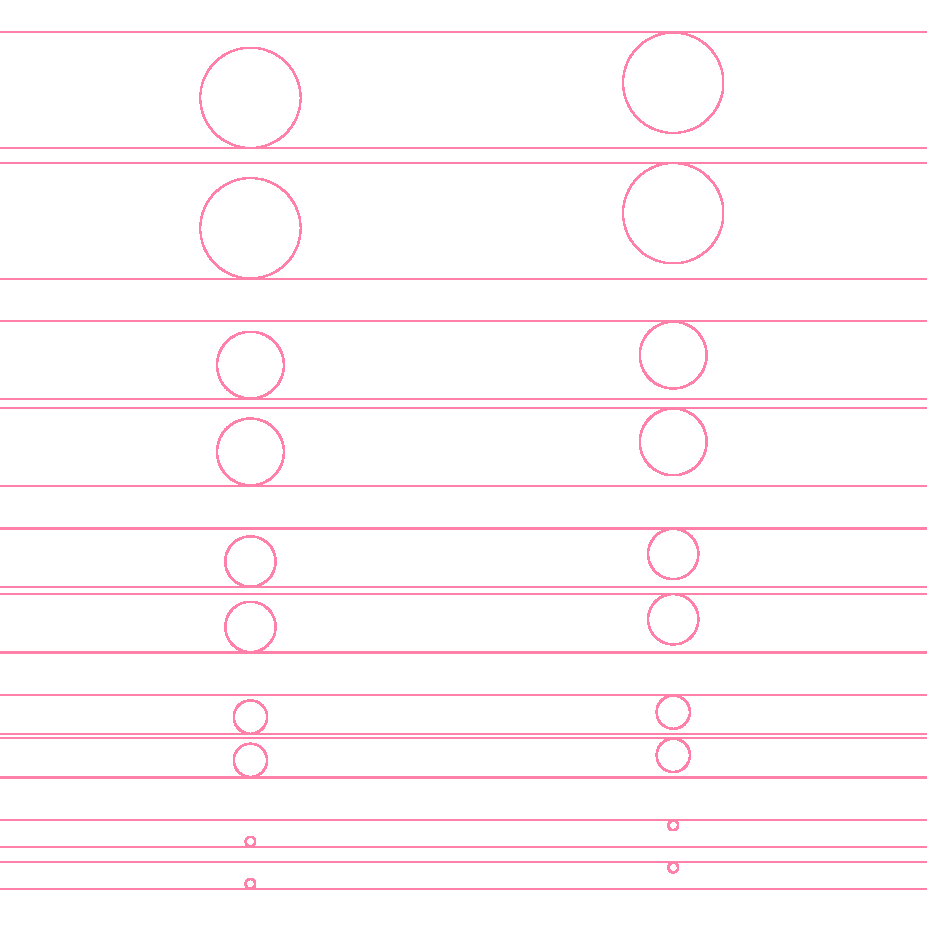
\includegraphics[width=.6\textwidth]{imgs/png/ligentec_gds}
	\caption{Caption}
	\label{fig:gds_ligentec}
\end{figure}

\begin{figure}
	\centering
	\begin{subfigure}[b]{0.45\textwidth}
		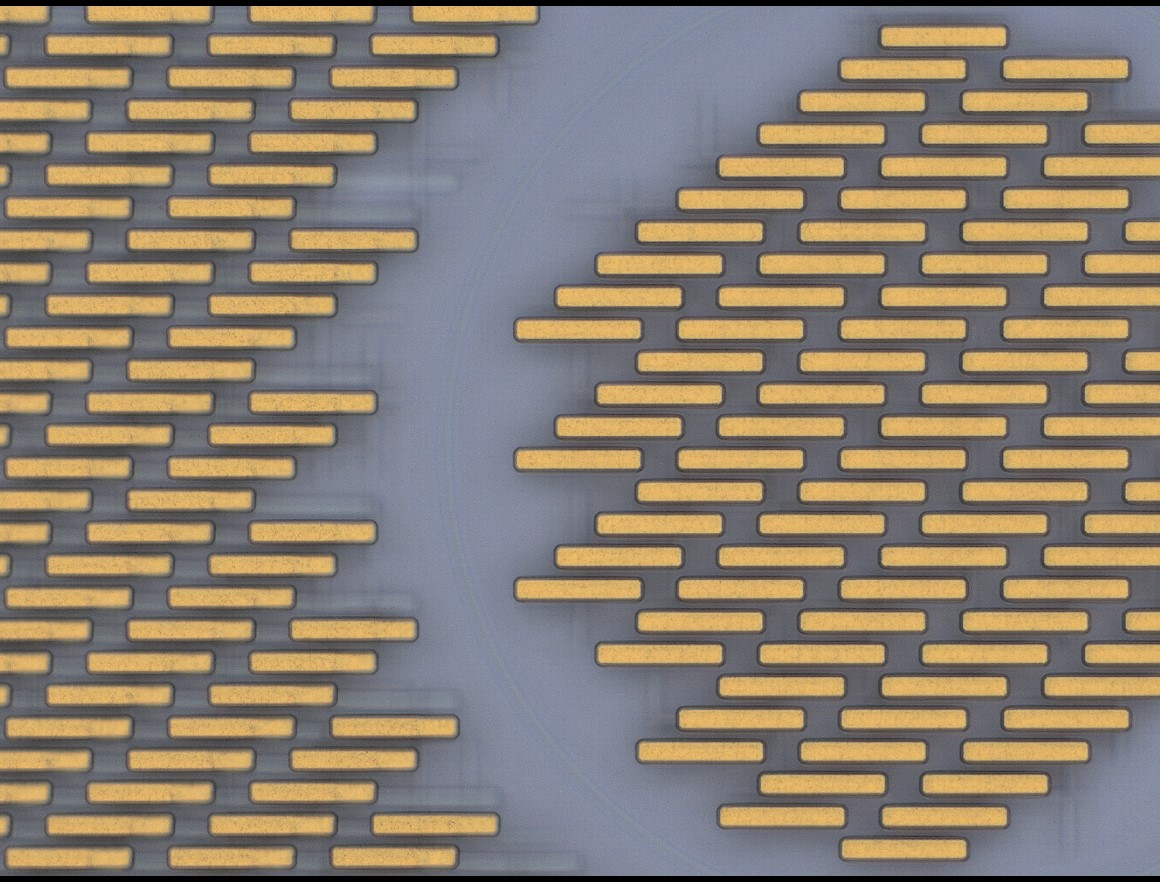
\includegraphics[width=\textwidth]{imgs/jpg/ligentec/top}
		\caption{}
	\end{subfigure}
	\begin{subfigure}[b]{0.45\textwidth}
		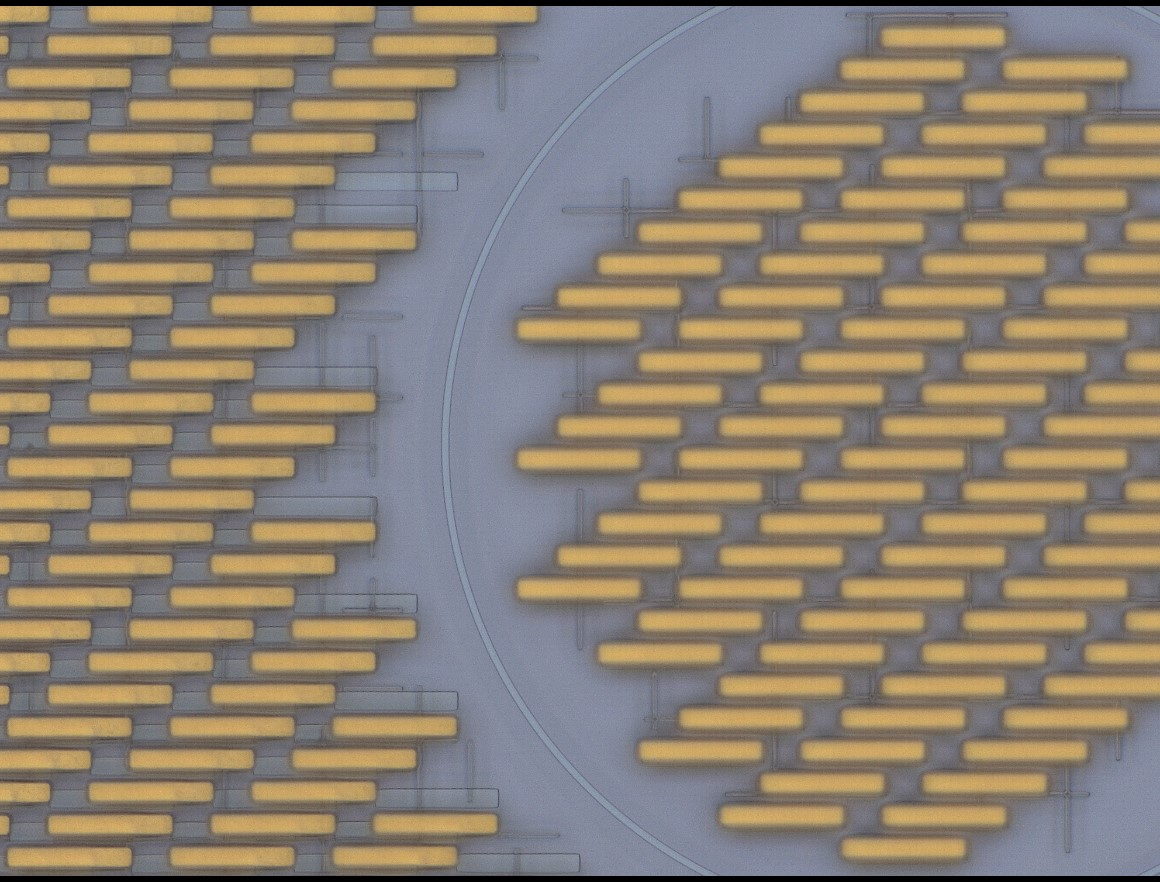
\includegraphics[width=\textwidth]{imgs/jpg/ligentec/dev}
		\caption{}
	\end{subfigure}
	\begin{subfigure}[b]{0.45\textwidth}
		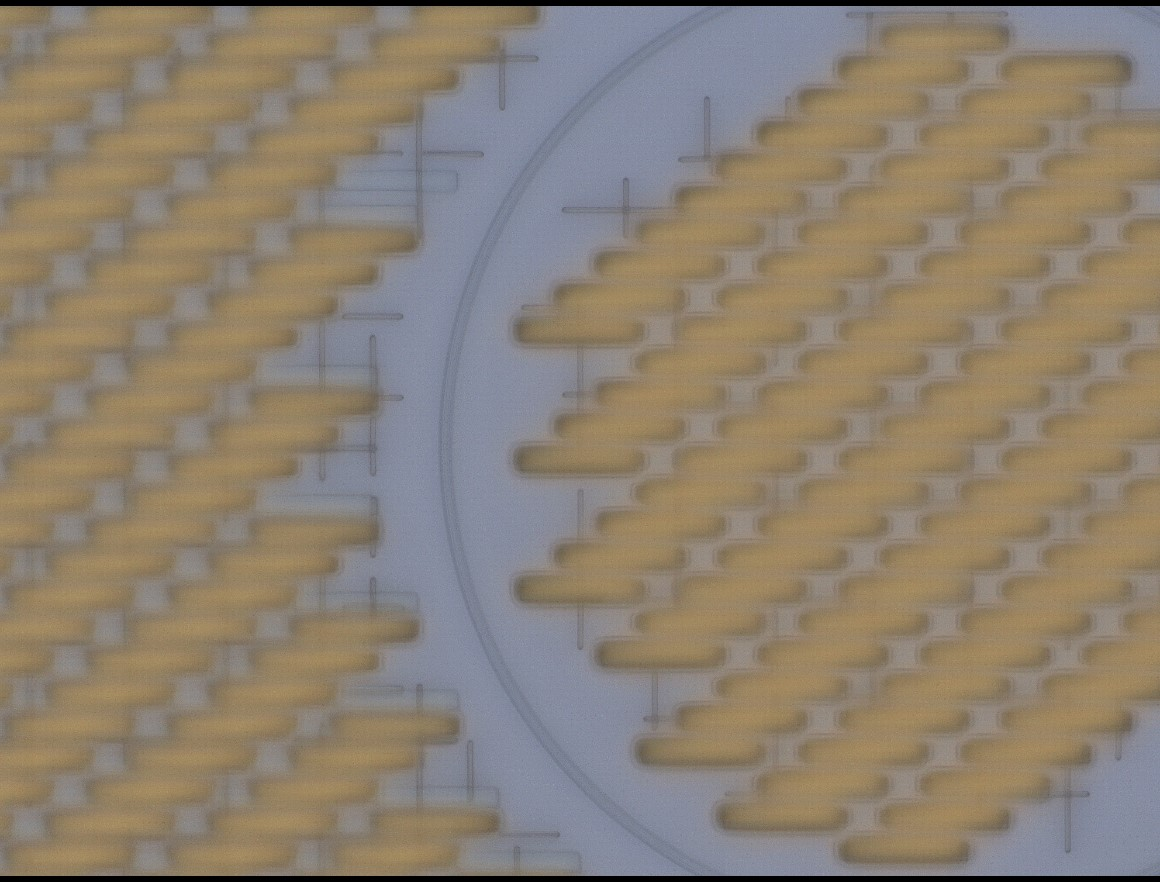
\includegraphics[width=\textwidth]{imgs/jpg/ligentec/cross}
		\caption{Crack stopper layer}
	\end{subfigure}
	\begin{subfigure}[b]{0.45\textwidth}
		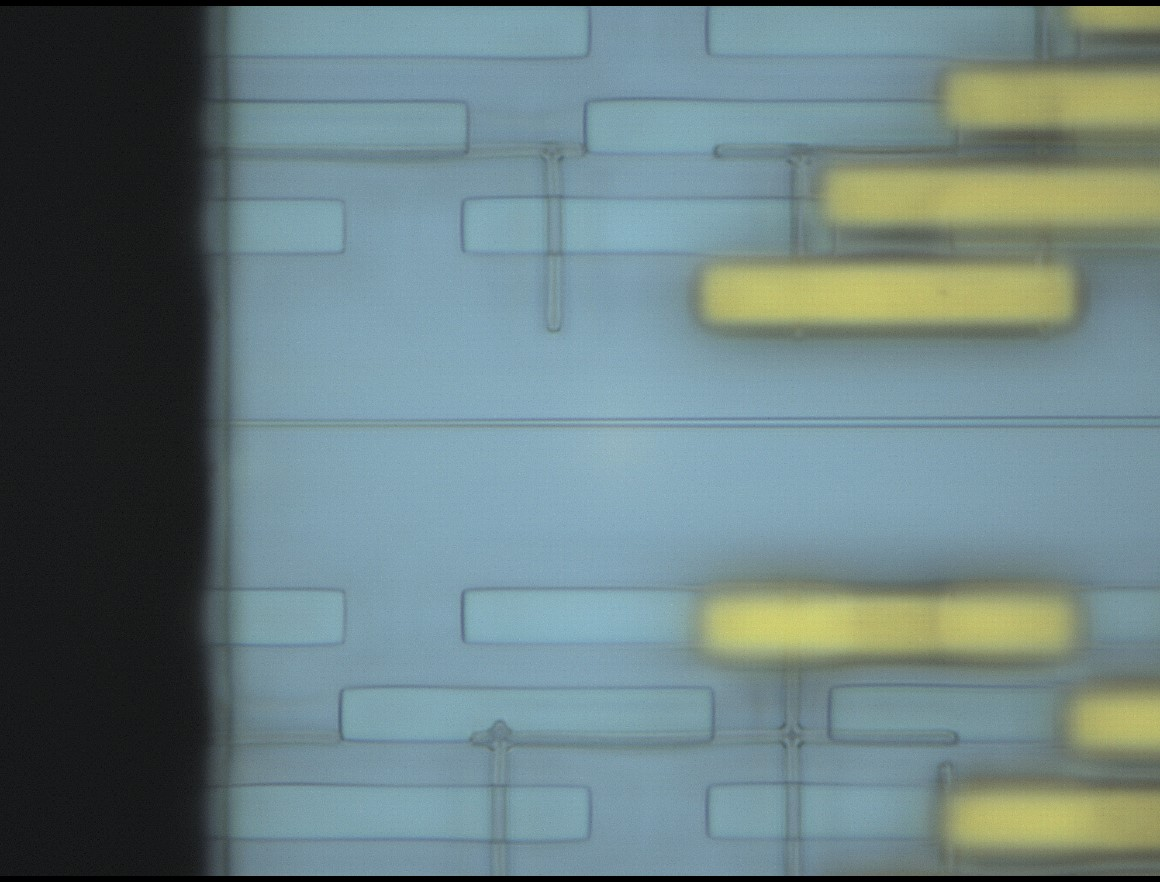
\includegraphics[width=\textwidth]{imgs/jpg/ligentec/cov}
		\caption{}
	\end{subfigure}
	\mycaption{Laser microscope images of Ligentec smaples}{By lowering the focus depth, three layers are observed.
		\textbf{a}. Top metallic layer. \textbf{b}. Device layer. \textbf{c}. Crack stopper layer. \textbf{d}. Mode convertor}
	\label{fig:ligentec-laser-micro}
\end{figure}

\section{NTT-AT technique}


NTT-AT technique adopts a different physical vapor method--reactive sputtering to deposit non-hydrogen silicon nitride. Compared with standard silicon sputtering, the nitrogen flow is supplied and reacts with silicon vapor into the silicon nitride film. The refractive index of the film deposited using method is also shown in \autoref{fig:ellipso}.

In the term design, the 4-inch wafer is customed with 22 cell in the layout shown in \autoref{fig:gds_ntt}, including the same design of Ligentec one in the special cell.

\begin{figure}
	\centering
	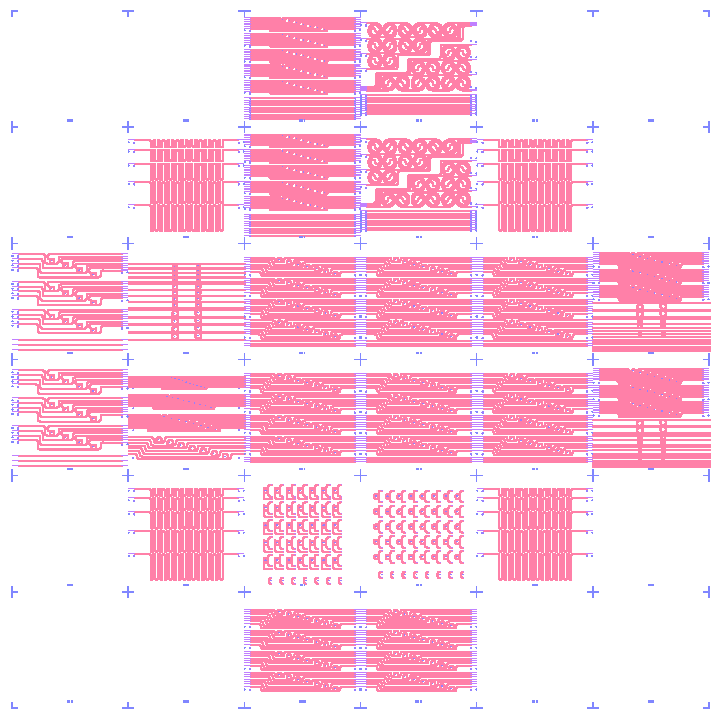
\includegraphics[width=\textwidth]{imgs/png/ntt_gds.png}
	\caption{Caption}
	\label{fig:gds_ntt}
\end{figure}


\section{Device evaluation}

\subsection{Coupling evolution}

Prior to cavity properties evaluation, it is essential to compare the coupling condition among devices in the same group. Since the gap between bus waveguide and ring resonator is swept increasingly, usually the coupling condition turns from over coupling to critical coupling, and finally into weak coupling.

For the Ligentec group 1, due to the reliable fabrication recipe, such an evolution of coupling condition among the same group is explicit as the gap increases.
As presented in \autoref{fig:gap_cf}(a), the coupling condition varies from over coupling to critical coupling, as the negative prominence of resonance peak increases. The same tendency agrees with the \textit{Q}-factors, shown in \autoref{fig:gap_cf}(b). The other groups in the sample have the similar tendency but the critical coupling gaps are different.

\begin{figure}
	\centering
	\includesvg[width=6in]{ligentec/gap_cf}
	\mycaption{Gap sweeping}{}
	\label{fig:gap_cf}
\end{figure}

\subsection{Quality factor comparison}


Several works using the same Ligentec technique report ultrahigh Q-factors up to \num{3d6} \cites{Yu2019, Vaidya2019}. The same magnitude is also attained in our samples in Group3 and Group5. While to compare the fabrication quality of both technique, two device with the same design (Group1 Device4, gap 700nm, FSR 100 GHz, ring width 0.8 \um ) are listed in \autoref{fig:fabless_cf}, as well as the \textit{Q}-factor histograms.

\begin{figure}
	\centering
	\includesvg[width=4in]{fabless_cf}
	\mycaption{A comparison between identical ring resonator fabricated in Ligentec and NTT-AT technique}{}
	\label{fig:fabless_cf}
\end{figure}

In the transmission of Ligentec device, shown in \autoref{fig:fabless_cf}(a)  and NTT-AT device shown in \autoref{fig:fabless_cf}(b), there is no obvious absorption in the range 1520 nm - 1540 nm compared with the samples fabricated using non-annealing subtractive recipe, though the transmission background declines at both red and blue side. However, the quality factors of Ligentec one are almost 4 times of NTT-AT samples, indicating the intracavity loss is 4 times lower. The histogram gathered in \autoref{fig:fabless_cf}(c) and \autoref{fig:fabless_cf}(b) features the same result.
In both samples, the critical coupling features at shorter wavelength, according to the peak prominence and \textit{Q}-factor tendency. 

We assume that despite the ammonia-free recipe used in NTT-AT technique, the etching recipe is not as fully optimized as Ligentec ones. It is also interesting to find that there is a clear difference of FSR trends from the former. In particular, the increasing NTT-AT FSRs indicate a normal dispersion.

%Besides, only fundamental mode is extracted from the transmission
%The device with deeper peaks are picked to locate the resonant wavelength, may not the minimum width though. 
%\autoref{fig:ligentec_triplot} presents the device transmission of group1 device 4, as well as quality factors and FSRs. The ring of this device is 237.28 \um and the FSR is targeted as 150 GHz.
%\begin{figure}
%    \centering
%    \includesvg[width=5in]{ligentec/ligentec_triplot}
%    \caption{Caption}
%    \label{fig:ligentec_triplot}
%\end{figure}

%In general, the waveguide width in the two device mentioned above is 0.8 \um. From the dispersion map in \autoref{fig:wg-disp}, waveguide in this size behave abnormal 
%\begin{figure}
%    \centering
%    \includesvg[width=5in]{ntt/ntt_triplot}
%    \caption{Caption}
%    \label{fig:ntt_triplot}
%\end{figure}

